\section{Physical model and free-energy functional}\label{sec:model}
We study a one-dimensional altermagnetic superconductor in the Nambu basis
\[\Psi_k=(c_{k+q/2,\uparrow},c_{k+q/2,\downarrow},c^\dagger_{-k+q/2,\uparrow},c^\dagger_{-k+q/2,\downarrow})^T\] with
\begin{equation}
H_{\rm BdG}(k)=\begin{pmatrix}h(k+q/2)-\mu&\Delta_q\\ \Delta_q^*&-\sigma_y h^T(-k+q/2)\sigma_y+\mu\end{pmatrix}.
\end{equation}
where $h(k)=t\cos k+(0,\lambda_y\sin k,\lambda_z\sin k+J_A\cos k)\cdot\boldsymbol\sigma$.
The production code evaluates the normal-referenced occupation-weighted spectral objective
\begin{align}
F_{\rm impl}(\Delta,q)={}&\frac{1}{2N_k}\sum_{k,n}E_n(k;\Delta,q)
f\!\left[\frac{E_n(k;\Delta,q)}{k_BT}\right]+\frac{\Delta^2}{U}\notag\\
&-\frac{1}{2N_k}\sum_{k,n}E_n(k;0,q)
f\!\left[\frac{E_n(k;0,q)}{k_BT}\right].
\end{align}
with $f(z)=1/(e^z+1)$ implemented as a stable sigmoid.  The sum includes all four BdG eigenvalue branches, the factor $1/2$ accounts for Nambu doubling, and the final term subtracts the $\Delta=0$ spectrum at the same $q$.  The $k$ sum is divided by the configured full grid size $N_k=800$.  Temperature enters only through the occupations: the production implementation contains no separately added entropy or log-partition term.  We therefore use $F_{\rm impl}$ for the implemented objective rather than replacing it by a textbook grand-potential expression.  All frozen minima and labels are those obtained from this objective, with energies in units of $t$.

\begin{table}[tb]\caption{Physical and numerical parameters.}\label{tab:s1}\centering
\begin{tabular}{lll}\toprule Quantity & Value & Role\\\midrule
$t$ & 1 & energy unit\\ $\lambda_y,\lambda_z$ & 0.6, 0.6 & spin--orbit couplings\\ $\mu$ & 0.55 & 2D chemical potential\\ $U$ & 1.6 & pairing interaction\\ $\omega_D$ & 10 & momentum mask cutoff\\ $N_k$ & 800 & Brillouin-zone grid\\ coarse $\Delta$ grid & $[0,0.6]$, 400 points & thermodynamic scan\\ initial $q$ grid & $[-1,0.5]$, 400 points & momentum scan\\ $\Delta_\epsilon,q_\epsilon$ & $10^{-3},10^{-2}$ & phase assignment\\\bottomrule\end{tabular}\end{table}

\section{Exact BdG oracle}
\refstepcounter{algorithm}\label{alg:oracle}\paragraph{Algorithm \thealgorithm: Thermodynamic and topology evaluation.}
\textbf{Input:} requested coordinate, numerical configuration, and enabled oracle mode.\par\textbf{Output:} observables, phase label, numerical status, and applicable topology fields.
\begin{enumerate}
\item For each coordinate, construct the BdG spectra on the configured $(\Delta,q)$ grid and evaluate the unchanged objective in Sec.~\ref{sec:model}.
\item Locate candidate minima. In the adaptive-box path, test enclosure; while allowed and necessary, expand the $q$ window directionally (at most three expansions). Refine selected global, nearly degenerate, and edge-risk basins using the configured grids (at least 800 $q$ and 600 $\Delta$ points in this path).
\item Apply the near-zero-$\Delta$ comparison. Assign thermodynamic identity separately from training eligibility and unresolved/rerun flags; the incremental oracle follows its recorded refinement configuration.
\item If the topology calculation is enabled and thermodynamic/numerical applicability holds, scan the full-zone gap. Only a resolved gapped FFLO state receives the Pfaffian index; otherwise return the relevant applicability or unresolved status.
\item Return records with numerical metadata. Coordinate reconciliation occurs at dataset merge; it is not a physical classification rule.
\end{enumerate}


\section{Reliability-state hierarchy}
Accepted/reliable points have an enclosed minimum and a resolved normal-state comparison. Boundary-delicate points lie within the adopted finite energy or order-parameter resolution. A $q$-window-unresolved point retains low-energy structure at the scanned edge after allowed expansion; a near-zero-$\Delta$-unresolved point lacks a resolved condensation-energy sign. Rerun-required records remain outside the clean physical training view. Topology-inapplicable includes all non-FFLO or numerically unreliable states, while gap-unresolved states do not receive a $\mathbb Z_2$ label. Phase identity, training eligibility, rerun status, and topology applicability are separate fields.
\begin{figure}[tb]\centering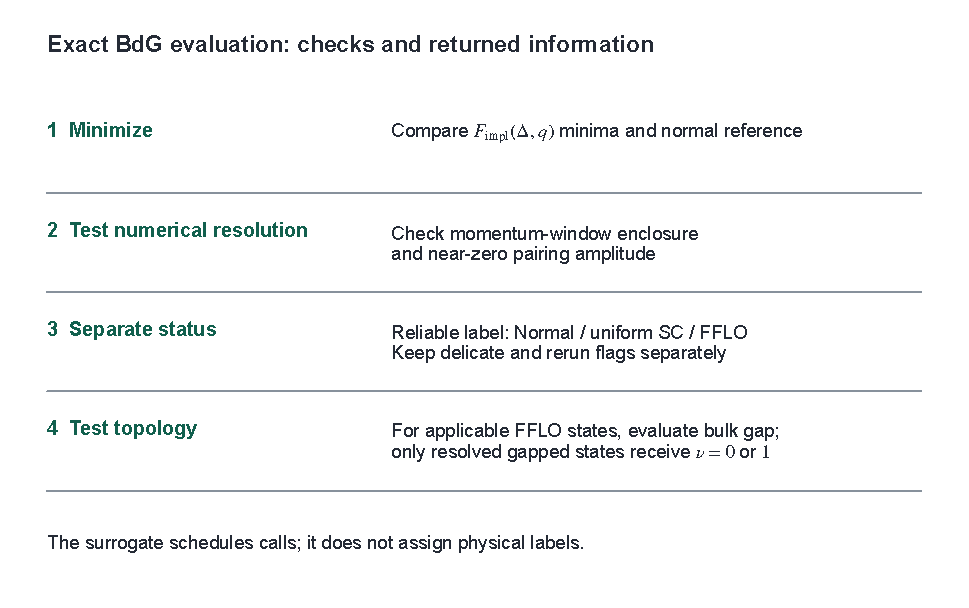
\includegraphics[width=\columnwidth]{figures/S1_reliability_flow.pdf}\caption{Exact-oracle reliability-state flow.  Numerical status is separate from phase identity, and topology is restricted to reliable gapped FFLO states.}\end{figure}

\section{Complete active-learning loop}
\refstepcounter{algorithm}\label{alg:loop}\paragraph{Algorithm \thealgorithm: Stage-resolved active-learning loop.}
\textbf{Input:} stage configuration and initial or resumed exact dataset (Sec.~\ref{sec:stage-settings}).\par\textbf{Output:} updated records, trained models, selected-call tables, and diagnostic history.
\begin{enumerate}
\item For a cold start, evaluate the stage-specific initial design; for a continuation, load the recorded resume dataset without drawing another seed.
\item At each iteration, construct the eligible training view and phase-stratified training/validation split. Reinitialize and train both ensembles; standardize inputs and regression targets using training statistics.
\item Generate the stage-specific candidate domain, predict observables/probabilities, and score the candidates using Secs.~\ref{sec:acq-definitions} and \ref{sec:stage-selectors}.
\item Select a batch using Algorithm~\ref{alg:batch}; write the point shards. Evaluate the BdG oracle and preserve failed or unresolved returns as explicit records.
\item Merge the completed shards, reconcile duplicate coordinate keys, and update the eligible learning view without overwriting reliability flags.
\item Recompute the recorded monitoring diagnostics. Continue unless the configured operational stop or budget is reached; save the dataset, configuration, selections, and diagnostics before returning.
\end{enumerate}


\section{Surrogate architecture and training}
The implementation uses separate PyTorch ensembles for regression and phase classification, not a Gaussian process or tree model. For Stages I--III, each of five members is an MLP with two 64-unit hidden layers and ReLU activations. Inputs are standardized by the training mean and standard deviation. Regression targets $(\Delta,q,\eta,I_c^+,I_c^-)$ are also standardized; the regression loss is mean-squared error. The classifier uses cross entropy on Normal, uniform-SC, and FFLO labels. Adam uses learning rate $10^{-3}$ and weight decay $10^{-5}$, batch size 512, and 240 epochs for both tasks. Members use seeds $42+1000+i$ and $42+2000+i$ for regression and classification. Models are retrained from scratch at each scheduling step; no early-stopping rule is implemented in these model classes. Regression uncertainty is the member standard deviation; phase probabilities are averaged over members and converted to entropy and margin scores.
\begin{table}[tb]\caption{Two-dimensional surrogate and training hyperparameters (Stages I--III).}\centering\setlength{\tabcolsep}{5pt}\begin{tabular}{ll}\toprule Item&Value\\\midrule ensemble size&5 per task\\ hidden layers&2 $\times$ 64, ReLU\\ validation fraction&0.15, phase stratified\\ optimizer&Adam\\ learning rate / weight decay&$10^{-3}/10^{-5}$\\ epochs / batch size&240 / 512\\ regression loss&MSE\\ classification loss&cross entropy\\ uncertainty&member dispersion / averaged probabilities\\\bottomrule\end{tabular}\end{table}
\begin{figure}[tb]\centering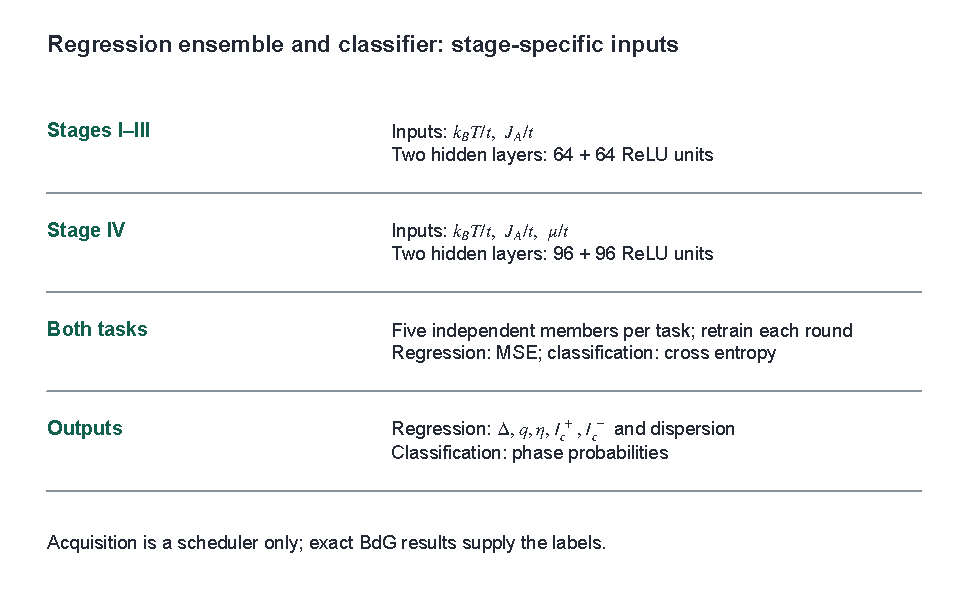
\includegraphics[width=\columnwidth]{figures/S2_surrogate_architecture.pdf}\caption{Stage-specific surrogate architecture. Stages I--III have two inputs and 64-unit hidden layers; Stage IV has three inputs and 96-unit hidden layers.  The regression and classification ensembles supply scheduling scores, not physical labels.}\end{figure}

\section{Acquisition function and microbatch selection}
Let $U_{\rm cls}=0.4H+0.6\exp[-m/0.2]$, where $H$ is normalized phase entropy and $m$ is the largest-probability margin. Let $U_{\rm reg}=(U_\Delta+U_q)/2$, $B_{NS}=\exp[-|\hat\Delta-\Delta_\epsilon|/0.04]\,4P_NP_{SC}$, $B_{UF}=P_{SC}\exp[-||\hat q|-q_\epsilon|/0.04]$, and $G=(G_\Delta+G_q)/2$.  The Stage-I/II full profile is
\begin{align} A_{\rm phase}&=U_{\rm cls}+0.6U_{\rm reg}+B_{NS}+0.9B_{UF}+0.5G,\notag\\ A_0&=A_{\rm phase}+0.4E_q+w_{\rm ext}E_{\rm ext}.\end{align}
where $E_q$ flags predicted $q$-edge risk and $E_{\rm ext}$ combines extrapolation with uncertainty. $w_{\rm ext}$ decreases piecewise from 0.15 to 0.08 and 0.03 at iterations 10 and 30. High-confidence interiors receive a soft penalty; the active pool is set by the larger of a scheduled quantile and $0.7p_{95}(A_0)$.  Observation repulsion uses length 0.02 and floor 0.5. During greedy stochastic construction, batch repulsion uses length 0.03 and floor 0.01, yielding $A_{\rm select}=A_{\rm pool}R_{\rm obs}R_{\rm batch}$ and sampling probability proportional to $A_{\rm select}^\gamma$, with $\gamma=1.5,2.5,4.0$ across the same schedule. Existing exact coordinates are excluded before selection.
\refstepcounter{algorithm}\label{alg:batch}\paragraph{Algorithm \thealgorithm: Stage-specific repelled selection.}
\textbf{Input:} candidate coordinates, component scores, existing observations, and stage configuration.\par\textbf{Output:} ordered selected batch, probabilities, and selection metadata.
\begin{enumerate}
\item In 2D, apply exact-coordinate and cooldown masks, interior penalties, and the active-pool threshold. Initialize batch repulsion to one and include observation repulsion.
\item In 3D, use the proposal pool and channel quotas; use the weighted combined score for exhausted-channel backfill. Apply the recorded duplicate handling.
\item While the requested batch is incomplete and positive finite weights exist: form the appropriate score times repulsion, raise to the stage-specific power, normalize, and sample one index.
\item Record its probability, remove the selected index, and multiply the remaining batch factors by $K(d;\ell,r)$. Return early if no eligible weight remains; do not invent extra oracle evaluations.
\end{enumerate}


\begin{table*}[t]\caption{Production acquisition components.}\centering\setlength{\tabcolsep}{5pt}\begin{tabular}{llll}\toprule Component&Definition&Normalization or weight&Role\\\midrule phase entropy/margin&$U_{\rm cls}$&0.4/0.6 mixture&classification ambiguity\\ regression spread&$U_{\rm reg}$&min--max normalized; 0.6&phase-facing uncertainty\\ Normal--SC&$B_{NS}$&competition gated; weight 1&order-parameter boundary\\ uniform--FFLO&$B_{UF}$&SC gated; weight 0.9&finite-$q$ boundary\\ gradients&$G$&grid derivative; weight 0.5&rapid variation\\ numerical risk&$E_q$&weight 0.4&$q$-window risk\\ exploration&$E_{\rm ext}$&annealed 0.15/0.08/0.03&domain coverage\\ repulsion&$R_{\rm obs}R_{\rm batch}$&length/floor rules&avoid redundant calls\\\bottomrule\end{tabular}\end{table*}
\begin{figure}[tb]\centering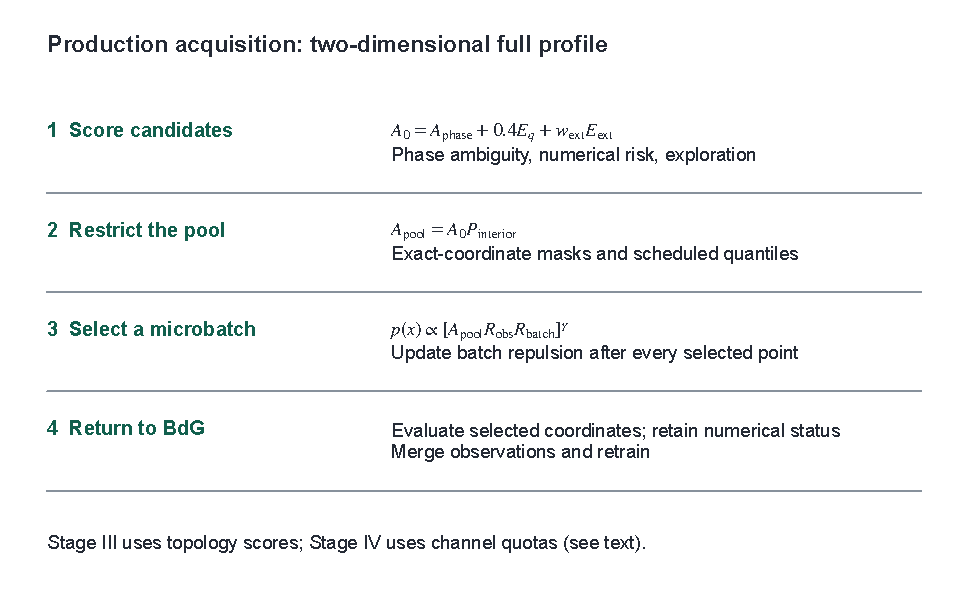
\includegraphics[width=\columnwidth]{figures/S3_acquisition_decomposition.pdf}\caption{Acquisition decomposition and repelled microbatch selection.}\end{figure}

\subsection{Stage-specific settings and auxiliary responses}\label{sec:stage-settings}
The run configurations distinguish initialization from continuation. Stage I uses a 512-location random-grid design, seed 42, on the $241\times321$ temperature--exchange grid. Stage II continues that dataset rather than drawing another independent seed. Stage III starts a separate 512-point scrambled Sobol design, also with seed 42, on the same bounded two-coordinate domain. Its final saved configuration is a resume at iteration 17; the initialization field describes the original run, not 512 additional observations at resume. Stage IV starts 1,024 scrambled Sobol points with seed 20260623 in the three-coordinate domain. The nominal subsequent batch size is 256 in all four stages; actual selected and retained counts need not equal this request.

\begin{table}[tb]\centering\setlength{\tabcolsep}{5pt}
\caption{Stage-specific training settings extracted from saved run configurations and the corresponding archived model constructors. Optimization batches are distinct from 256-point oracle batches.}\label{tab:networks}
\begin{tabular}{lccc}\toprule Setting & Stages I--II & Stage III & Stage IV\\\midrule
Input coordinates & $T,J_A$ & $T,J_A$ & $T,J_A,\mu$\\
Hidden layers (ReLU) & $64,64$ & $64,64$ & $96,96$\\
Members per task & 5 & 5 & 5\\
Epochs (regression/classification) & $240/240$ & $240/240$ & $180/180$\\
Optimization batch size & 512 & 512 & 512\\
Learning rate & $10^{-3}$ & $10^{-3}$ & $10^{-3}$\\
Weight decay & $10^{-5}$ & $10^{-5}$ & $10^{-5}$\\
Validation fraction & 0.15 & 0.15 & 0.15\\
Base seed & 42 & 42 & 20260623\\\bottomrule
\end{tabular}\end{table}
All stages train separate regression and classification ensembles. The archived Stage-IV adapter overrides the input dimension, hidden width, epoch count, ensemble size, and seed; its optimization batch size, Adam settings, and validation fraction come from the archived constructor, not from the current development defaults. The target vector remains $(\Delta_{\rm opt},q_{\rm opt},\eta,I_c^+,I_c^-)$. No additional learned spectral network is used in the Stage-III/IV acquisition implementation examined here: predicted $\Delta,q$ are passed to analytic Pfaffian expressions to construct scheduling proxies. They do not replace exact spectral labels.

Here $I_c^+\geq0$ and $I_c^-\leq0$ are the signed extrema located on the positive and negative current branches outward from the optimized momentum. The implementation records
\begin{equation}\eta=\frac{|I_c^+|-|I_c^-|}{|I_c^+|+|I_c^-|},\label{eq:eta}\end{equation}
with zero returned if both currents vanish (and $-1$ or $+1$ if only the positive or negative branch vanishes). These are auxiliary response targets, not independently validated diode-response claims. In the saved Stage-I/II \texttt{full} profile, response scores are exported but excluded from the main acquisition. Stage III's \texttt{topo\_trivial} profile and Stage IV's explicit three-channel selector likewise use the $\Delta,q$ uncertainty channels rather than $\eta,I_c^\pm$ to schedule calls. The presence of an optional response-weighted cleanup branch in the archived code is not evidence that it was used in these endpoint configurations.

\subsection{Definitions of the two-dimensional acquisition components}\label{sec:acq-definitions}
The following definitions apply to the saved two-dimensional implementation. Write $\mathcal N[z]=(z-z_{\min})/(z_{\max}-z_{\min})$ over finite values on the candidate array; constant arrays and nonfinite entries map to zero, and the result is clipped to $[0,1]$. Each uncertainty channel is normalized separately. Grid gradients use first-order edge differences and coordinate spacings, not pixel indices:
\begin{equation}
G=\tfrac12\mathcal N\!\left[\sqrt{(\partial_{T/t}\hat\Delta)^2+(\partial_{J_A/t}\hat\Delta)^2}\right]
+\tfrac12 P_{SC}\mathcal N\!\left[\sqrt{(\partial_{T/t}|\hat q|)^2+(\partial_{J_A/t}|\hat q|)^2}\right].\label{eq:gradient}
\end{equation}
In this equation the temperature coordinate denotes $k_BT/t$. Let $[z]_+=\max(z,0)$, $d_q=\min(|\hat q+1|,|0.5-\hat q|)$, and $\tau=k_BT/t$, $j=J_A/t$. Then
\begin{align}
E_q&=P_{SC}\max\{\exp[-d_q/0.02],\mathcal N([j-1.2]_+)\},\label{eq:eq-risk}\\
E_{\rm ext}&=\max\{\mathcal N([\tau-0.5]_+),\mathcal N([j-1.2]_+)\}\max\{U_{\rm cls},U_{\rm reg}\}.\label{eq:extrapolation}
\end{align}
The thresholds above are acquisition parameters, not physical phase criteria. The interior indicator requires $P_{\max}>0.98$ and each of $U_{NS}$, $U_{UF}$, $G$, $E_q$, and $E_{\rm ext}$ below 0.05, with $U_{NS}=4P_NP_{SC}$ and $U_{UF}=4P_{\rm uniform}P_{\rm FFLO}$. Its multiplicative penalty is 0.5 before iteration 10 and 0.1 afterward; all other candidates retain factor one. Thus $A_{\rm pool}=A_0P_{\rm interior}$, not the unpenalized score.

The pool quantile is 0.90, 0.95, and 0.98 before iteration 10, from 10 to 29, and from 30 onward. Among eligible hard-unseen candidates, the threshold is the maximum of this quantile and $0.7Q_{0.95}(A_{\rm pool})$. The target admitted fraction decreases linearly from 0.20 at iteration zero to 0.05 at iteration 30. If exceeded, the quantile increases in steps of 0.005, up to 0.995, subject to the minimum-batch guard; ties and this quantile ceiling mean this is not an unconditional exact cardinality cap. Before iteration 5, quantile relaxation in steps of 0.02 down to 0.70 may fill the configured minimum batch (64); afterward underfilled batches are allowed and no information-free filling is required.

Distances below use coordinates divided by their domain ranges, $(0.56,2.12)$, with $d_{\rm obs}$ the nearest retained-coordinate distance. The repulsion kernel and within-batch update are
\begin{align}
K(d;\ell,r)&=r+(1-r)\{1-\exp[-(d/\ell)^2]\},\label{eq:kernel}\\
R_{\rm obs}(x)&=K(d_{\rm obs}(x);0.02,0.5),\qquad
R_{\rm batch}(x;\mathcal B)=\prod_{s\in\mathcal B}K(d(x,s);0.03,0.01),\label{eq:repulsion}\\
p(x\mid\mathcal B)&=\frac{[A_{\rm pool}(x)R_{\rm obs}(x)R_{\rm batch}(x;\mathcal B)]^\gamma}
{\sum_{z\in\mathcal P\setminus\mathcal B}[A_{\rm pool}(z)R_{\rm obs}(z)R_{\rm batch}(z;\mathcal B)]^\gamma}.\label{eq:batchprob}
\end{align}
Here $\mathcal P$ is the eligible active pool and $\gamma=1.5,2.5,4$ on the same iteration intervals. A selected index is removed immediately, and the product is updated after every pick. Existing exact coordinates are excluded using four-decimal coordinate keys; configured recent-selection and normal-boundary-band cooldowns also apply. Repeated requests in historical accounting must not be equated with successful unique returns.

\subsection{Topology-aware and three-dimensional selectors}\label{sec:stage-selectors}
Stage III replaces the \texttt{full} score by $w_p\mathcal N(A_{\rm phase})+w_sA_s+w_cA_c$, with weights $(0.45,0.45,0.10)$ before iteration 30 and $(0.25,0.65,0.10)$ thereafter. It does not simply add a new spectral head to the old full score. The spectral proxy is the maximum of a Pfaffian-margin score, an opposite-index proximity score, and a gapless-support proximity score. With normalized distances $d_0,d_1,d_g,d_t$ to trivial, topological, gapless, and trusted-topology observations,
\begin{align}
A_s&=P_{SC}\max\{e^{-m_P/0.02},e^{-\min(d_0,d_1)/0.06-|d_0-d_1|/0.06},e^{-d_g/0.06}\},\label{eq:toposcore}\\
A_c&=P_{SC}\{1-e^{-(d_t/0.08)^2}\}.\label{eq:topocoverage}
\end{align}
Absent support sets disable their proximity term; absent trusted-topology support gives $A_c=P_{SC}$. The dimensionless margin is $m_P=\min(|P_0|,|P_\pi|)/E_*^2$, with $E_*=\max(1,|t|,|\lambda_y|,|\lambda_z|,|\mu|,|J_A|,|\Delta|)$ in the code's energy units and a $10^{-300}$ denominator floor. Stage III uses the fixed chemical potential; Stage IV uses the candidate chemical potential. These scores guide selection and confer no topological label.

Stage IV constructs a nominal 65,536-point proposal pool: 70\% global scrambled Sobol, 10\% jittered local thermodynamic-bracket midpoints, 15\% jittered topology-bracket midpoints, and 5\% chemical-potential-edge proposals. Missing bracket proposals are backfilled. This is a different proposal strategy from Stage III's diagnostic-only brackets. Coordinates are clipped to the recorded domain and proposal duplicates are removed at eight decimal places. Existing observations are identified at six decimal places. The saved selection tables, not a nominal pool-size assumption, determine actual call counts.

The Stage-IV phase score is $\operatorname{clip}[0.65H+0.35\operatorname{clip}(\bar\sigma/Q_{0.95}(\bar\sigma),0,1),0,1]$, where $\bar\sigma=(\sigma_\Delta+\sigma_q)/2$ and the denominator has a $10^{-12}$ floor. Its spectral score takes the larger of the Pfaffian-margin term and the opposite-index term in Eq.~\eqref{eq:toposcore}, now with distance scale 0.08 and no gapless term. Coverage is $1-\exp[-(d_{\rm obs}/0.04)^2]$, without $P_{SC}$. Distances normalize all three domain ranges $(0.56,2.12,2.0)$.

Channel weights $(0.45,0.40,0.15)$ change to $(0.25,0.60,0.15)$ at iteration 12. The selector allocates integer phase/spectral/coverage quotas from these weights; within each channel it samples the channel score times batch repulsion to power 3. Exhausted channels fall back to the weighted combined score. Batch repulsion uses $\ell=0.045$, floor 0.02, and the same product update as Eq.~\eqref{eq:repulsion}. Thus Stage IV must not be described as the two-dimensional quantile-pool selector applied unchanged in three dimensions.

\section{Sampling efficiency}\label{sec:counts}
The Stage-I candidate universe is the complete $241\times321$ Cartesian grid over $k_BT/t\in[0,0.56]$ and $J_A/t\in[0,2.12]$, containing 77,361 locations.  Its endpoint contains 6,880 unique exact coordinates, so $f_{\rm exact}=6880/77361=0.08893$ and $R_{\rm call}=77361/6880=11.24$.  Stage II continues on the same candidate domain and contains every Stage-I endpoint coordinate plus 554 new exact coordinates, producing the 7,434-coordinate reliability endpoint displayed in main-text Fig.~\ref{main-fig:thermo}.  Shared coordinates have identical phase labels.  Selection records exceed endpoint coordinates because repeated requests and selected coordinates without a retained endpoint return are separate accounting layers.  A boundary-enrichment factor cannot be reconstructed because complete candidate-pool boundary labels are absent.  Per-iteration timings exist, but no matched exhaustive-grid baseline supports a wall-time speedup.
\begin{table*}[t]\caption{Stage-resolved selection and retained-coordinate accounting.}\label{tab:counts}\centering\setlength{\tabcolsep}{5pt}\begin{tabular}{lrrl}\toprule Quantity&Stage I&Stage II&Meaning\\\midrule prescribed candidate locations&77,361&77,361&common Cartesian domain\\ selected call records&8,192&9,216&requests, including repeats\\ unique selected coordinates&7,305&7,885&deduplicated requested locations\\ unique exact endpoint coordinates&6,880&7,434&retained exact observations\\ training-eligible records&6,880&7,434&clean learning view\\ trusted exact records&6,104&6,598&reliable subset\\ selected without endpoint record&425&451&no retained endpoint return\\\midrule sampling fraction&8.893\%&--&Stage-I discovery headline\\ exact-location reduction&11.244$\times$&--&grid locations, not wall time\\\bottomrule\end{tabular}\end{table*}
\begin{figure}[tb]\centering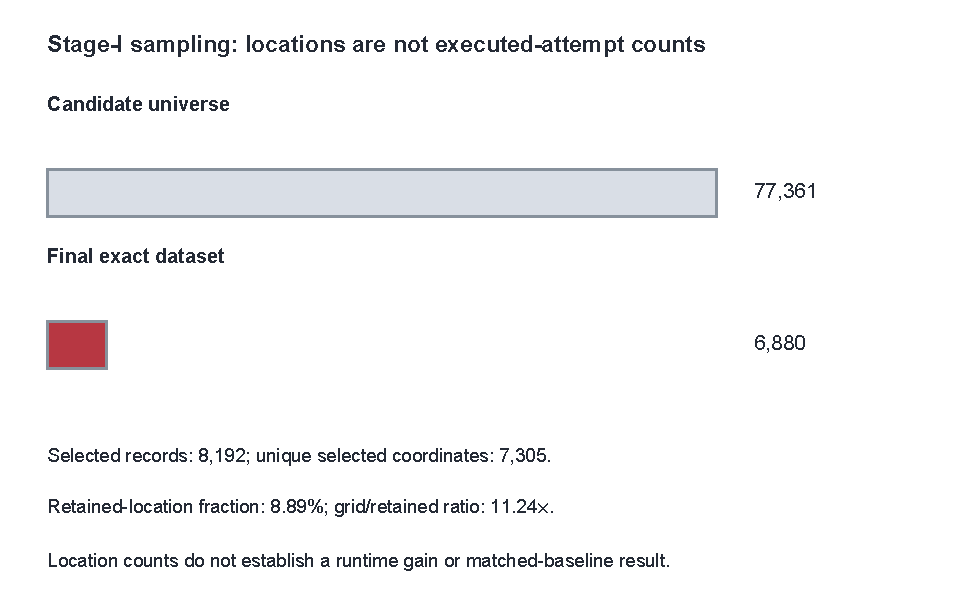
\includegraphics[width=\columnwidth]{figures/S4_sampling_efficiency.pdf}\caption{Stage-I candidate-universe and exact-location accounting.  The reduction is a location-count ratio, not a wall-time acceleration.}\end{figure}

\section{Numerical diagnostics and operational stopping}
These criteria are operational controls for the numerical workflow. They are not thermodynamic observables or universal physical scales. Phase-map change is the fraction of fixed monitor-grid cells whose predicted phase changes between iterations. Boundary displacement is a bidirectional nearest-neighbor $p_{95}$ distance between successive extracted boundary point sets after normalization by the parameter-domain ranges. Coverage is the $p_{95}$ distance from the current monitor-grid boundaries to exact samples. Surprise is the fraction of returned labels that differ from the prior prediction, with trusted and flagged denominators stored separately. Four of five main conditions must hold for four successive iterations after a five-iteration minimum. The adopted thresholds reflect the monitor-grid resolution and workflow tolerance, not a physical scale.
\begin{table*}[t]\caption{Operational diagnostics.}\centering\setlength{\tabcolsep}{5pt}\begin{tabular}{p{0.16\textwidth}p{0.20\textwidth}p{0.18\textwidth}p{0.17\textwidth}p{0.15\textwidth}}\toprule Diagnostic&Definition&Domain&Operational setting&Interpretation\\\midrule phase-map change&changed-cell fraction&fixed $241\times321$ monitor&$<0.002$&map stability\\ Normal--SC shift&bidirectional $p_{95}$&normalized domain&$<0.004167$&boundary stability\\ SC--FFLO shift&bidirectional $p_{95}$&normalized domain&$<0.004167$&boundary stability\\ coverage&boundary-to-exact $p_{95}$&normalized domain&$<0.00625$&sampling support\\ label surprise&prediction/return mismatch&selected calls&$<0.05$&sequential stability\\ patience&successive eligible iterations&iteration history&4&operational termination\\\bottomrule\end{tabular}\end{table*}

\section{Topology diagnosis and reconstruction sensitivity}\label{sec:topology}
Topology is applicable only to thermodynamically accepted, numerically reliable, gapped FFLO states.  The minimum absolute BdG eigenvalue is scanned over the full Brillouin zone.  At $k=0,\pi$, the analytic Pfaffians are
\begin{align}P_0={}&(\mu-t\cos(q/2))^2+\Delta^2-(\lambda_y\sin(q/2))^2\notag\\ &-(J_A\cos(q/2)+\lambda_z\sin(q/2))^2,\\ P_\pi={}&(\mu+t\cos(q/2))^2+\Delta^2-(\lambda_y\sin(q/2))^2\notag\\ &-(J_A\cos(q/2)+\lambda_z\sin(q/2))^2.\end{align}
Away from the relative Pfaffian tolerance $10^{-8}$, $P_0P_\pi<0$ gives $\nu=1$ and $P_0P_\pi>0$ gives $\nu=0$. Analytic values were checked against direct Majorana-basis Pfaffians, and CPU/GPU full-zone gaps were compared in the archived topology validation. The displayed transition contour is a deterministic support-restricted reconstruction on a $401\times401$ monitor grid with support radius 0.045.  For neighborhoods $k=6,8,12$, its arc lengths are 0.8270, 0.8215, and 0.8038, while coverage $p_{95}$ is 0.006269, 0.006185, and 0.005913. This sensitivity and the local opposite-$\mathbb Z_2$ brackets make the contour a guide to the gap-closing region rather than an exact boundary; nodal alternatives are not exhaustively excluded.

\section{Three-dimensional extension}\label{sec:3d}
Stage IV samples $(k_BT/t,J_A/t,\mu/t)$ with $\mu/t\in[-0.5,1.5]$. The main figure shows the exact thermodynamic point cloud, reliable FFLO topology support, and bins centered at $\mu/t=-0.45,0.15,0.85,$ and $1.45$ with half-width 0.025. No interpolation is performed between these bins. Archived map-change, proxy-surface displacement, coverage, surprise, and component-count histories are retained as numerical diagnostics only. The discrete support reveals systematic three-dimensional structure but does not establish a converged continuous topology surface or complete atlas.


\begin{table}[tb]\centering\caption{Main-text Fig.~\ref{main-fig:3d}(c) bin accounting. Each window has half-width 0.025. Trusted here is the numerical-reliability subset, not the gapped-FFLO topology subset.}\label{tab:bins}
\begin{tabular}{rrrrrr}\toprule $\mu/t$ center & Retained & Normal & Uniform SC & FFLO & Trusted\\\midrule
$-0.45$&272&95&1&176&255\\$0.15$&154&53&4&97&149\\$0.85$&223&57&18&148&208\\$1.45$&142&104&3&35&139\\\bottomrule\end{tabular}\end{table}
Main-text Fig.~\ref{main-fig:topology}(a) contains 3,213 trusted gapped FFLO observations (2,290 cFFLO and 923 tFFLO). The main-text reconstruction retains the $k=8$ operational-audit pass and the $k=6$ sensitivity deviation; neither is a universal physical convergence criterion. The four three-dimensional bin totals in Table~\ref{tab:bins} count retained observations, not estimates of phase-space volume.
\begin{figure}[tb]\centering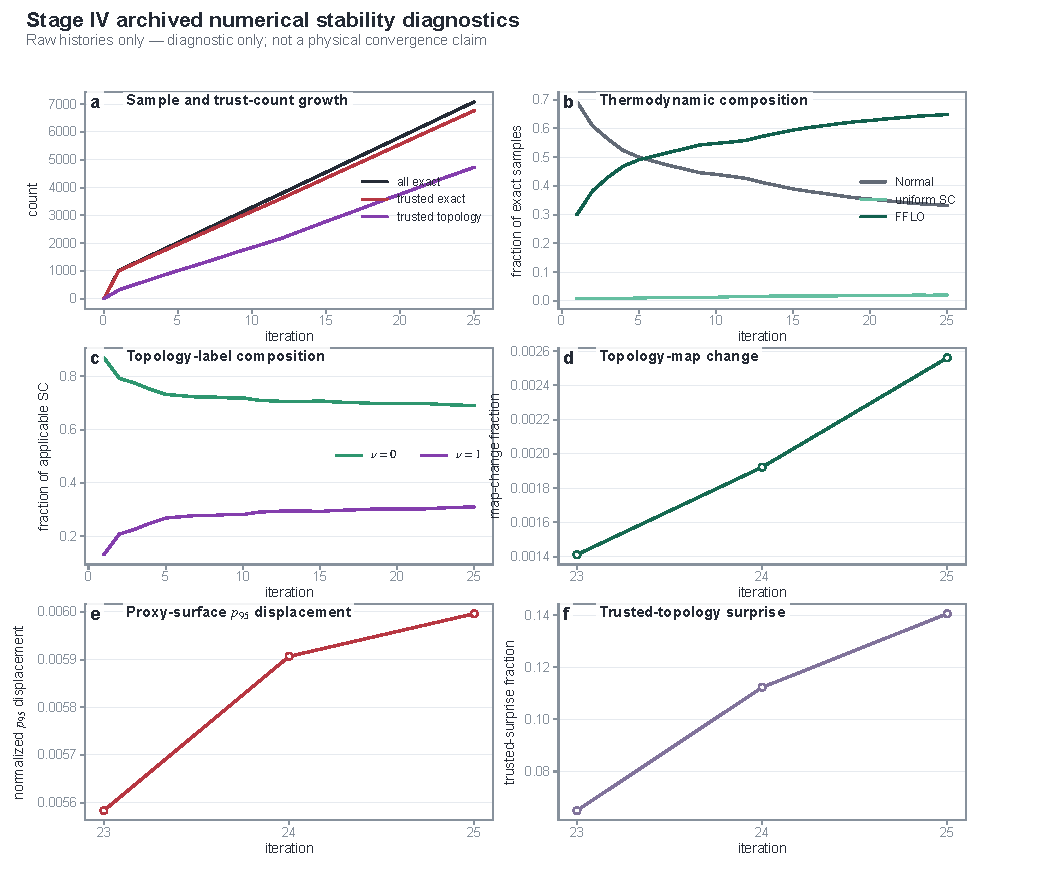
\includegraphics[width=\textwidth]{figures/sm_stageiv_numerical_diagnostics.pdf}
\caption{Stage-IV numerical histories, without threshold lines. (a) Retained and trusted sample growth. (b) Thermodynamic composition. (c) Topology composition. (d) Available topology-map changes. (e) Proxy-surface displacement. (f) Trusted-label surprise. These are iteration diagnostics, not a formally converged three-dimensional topology surface.}\label{fig:3d-diagnostics}\end{figure}
\section{Reproducibility, code, data, and environment}\label{sec:reproduction}
The scientific entry points and the manuscript build serve different purposes. The historical two-dimensional run configuration identifies \path{scripts/slurm_exact_oracle_array.sh} for pointwise jobs; active-learning preparation is implemented in \path{ml_phase/active_refine.py}. The corresponding archived modules include \path{ml_phase/exact_oracle.py}, \path{models.py}, \path{acquisition.py}, and \path{topology_oracle.py}. The three-dimensional launch package contains \path{scripts/submit_stageiv_3d_full_loop.sh}, \path{scripts/stageiv_3d_select.py}, and \path{scripts/slurm_stageiv_exact_array.sh}; selection calls \path{ml_phase/stageiv_3d.py} with the saved production configuration. These identify scientific entry points, not a claim that running a LaTeX script repeats the physical calculations.

The export contains archived source snapshots and run configurations, not a public executable service. Stages I--III record Python 3.10.20 and PyTorch 2.11.0+cu130, with eight round-robin oracle shards. These environment and deployment entries should not be generalized to all runs: the Stage-IV launch script defaults to eight cost-aware shards and CPU selection, but shell overrides and the complete deployment environment are not established by the production JSON alone. Reproduction additionally requires the launch package, actual job overrides, and platform setup. Bitwise GPU reproducibility is not established by a fixed pseudorandom seed alone.

The retained datasets, selection tables, and numerical histories underlie the main figures. In particular, main-text Fig.~\ref{main-fig:thermo} uses the Stage-II retained-coordinate dataset, Fig.~\ref{main-fig:topology} uses the reliable gapped FFLO subset and support-restricted reconstruction, and Fig.~\ref{main-fig:3d} uses the Stage-IV point cloud with the bin convention in Sec.~\ref{sec:3d}. Table~\ref{tab:counts} separates requests, unique requested locations, and retained observations. Total executed evaluations, including failed attempts and repeat work, cannot be inferred from these three counters alone; no complete executed-attempt ledger is claimed here.

The accompanying document-source package contains a separate \path{build.py} that regenerates the double-column main text, single-column review text, and this Supplement from a clean temporary directory. This script only builds documents from unchanged figure assets. Input hashes identify the source versions because the local export contains no Git repository metadata. Neither the archived scientific package nor these manuscript sources have a confirmed public repository URL or persistent identifier; public access and long-term deposition remain to be arranged by the authors.

Saved run configurations establish the stage-specific parameter choices, while the export provides shared and stage-specific source snapshots. A per-run commit or executable hash linking every Stage-I/II invocation to the shared source snapshot is not available in this package. Accordingly, the method descriptions document the recovered implementation and recorded configurations; they are not a demonstrated end-to-end rerun or a complete executed-attempt ledger.
